\chapter{Design Principles}

\section{Introduction to Shneiderman's Mantra}

In the realm of information visualization, effective data exploration is really important. Ben Shneiderman, a prominent figure in human-computer interaction, proposed a foundational guideline known as Shneiderman's Mantra to improve user interaction with complex datasets. The mantra states: \textit{"Overview first, zoom and filter, then details-on-demand"} \cite{hampdatavisualizationSchneidermansMantra2016}. This principle stands as a blueprint for designing intuitive interfaces that hold efficient data analysis.

Shneiderman's Mantra emphasizes a hierarchical approach to data exploration:

\begin{enumerate} 
    \item \textbf{Overview First}: Present the entire dataset in a high-level view to provide context and scope. \item \textbf{Zoom and Filter}: Allow users to focus on subsets of the data that interest them. 
    \item \textbf{Details on Demand}: Enable access to detailed information about specific data points when required. 
\end{enumerate}

This sequence allows interfaces to cater to both regular users and experts and provide scalable means to interact with data of varying complexity.

\section{Implementation in the Birds of Sweden Dashboard}

I developed the Birds of Sweden Dashboard in this course to enable users to navigate and explore Sweden's bird fauna interactively. Implementing Shneiderman's Mantra within this dashboard makes sure that users can effectively analyze bird observation data across the country.

\subsection{Overview First}

Upon launching the dashboard, users are presented with a comprehensive map displaying all bird observations across Sweden (Figure~\ref{fig:overview}). This initial view provides an immediate sense of the spatial distribution and density of bird sightings which fulfills the "Overview First" principle.

\begin{figure}[h] 
    \centering 
    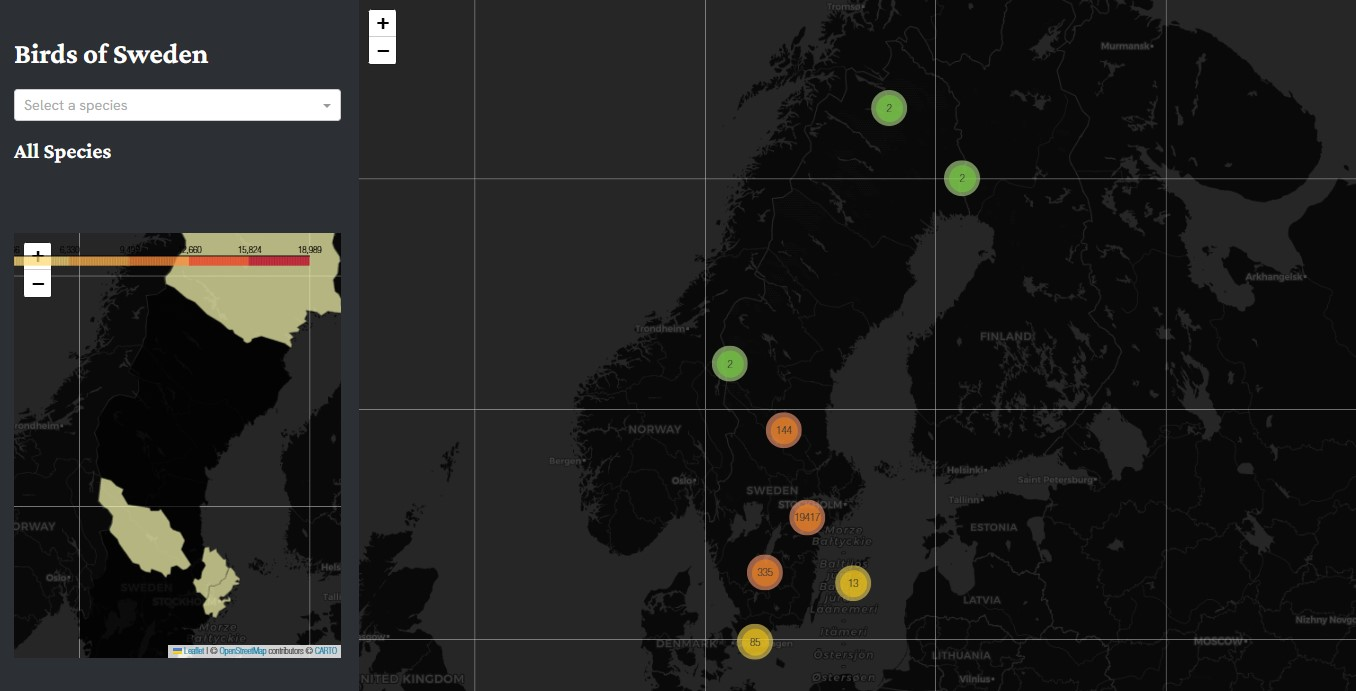
\includegraphics[width=0.8\textwidth]{figures/overview_map.jpg} 
    \caption{Initial overview of all bird observations in Sweden.} 
    \label{fig:overview} 
\end{figure}

The map utilizes a scatter plot where each point represents an observation, allowing users to perceive patterns such as hotspots of biodiversity or migratory pathways. Additionally, the sidebar includes a state observations map that consistently displays the entire country's outline, highlighting the number of observations per state. This reinforces the comprehensive nature of the overview.

\subsection{Zoom and Filter}

To facilitate more focused exploration, the dashboard incorporates interactive filtering mechanisms. A dropdown menu enables users to select a specific bird species from an extensive list derived from the dataset (Figure~\ref{fig:dropdown}). Upon selection, the main map updates to display only the observations pertaining to the chosen species.

\begin{figure}[h] 
    \centering 
    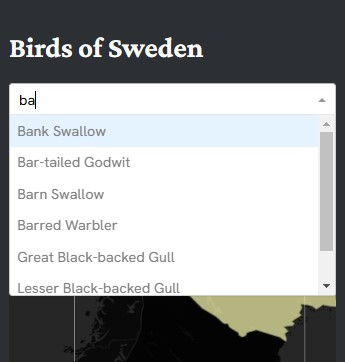
\includegraphics[width=0.4\textwidth]{figures/species_dropdown.jpg} 
    \caption{Species selection dropdown for filtering observations.} 
    \label{fig:dropdown} 
\end{figure}

This filtering capability exemplifies the "Zoom and Filter" principle, allowing users to narrow down the dataset to areas or species of interest. The state observations map in the sidebar also updates accordingly, highlighting only the states where the selected species has been observed, thus providing a filtered geographical context (Figure~\ref{fig:filtered_map}).

\begin{figure}[h] 
    \centering 
    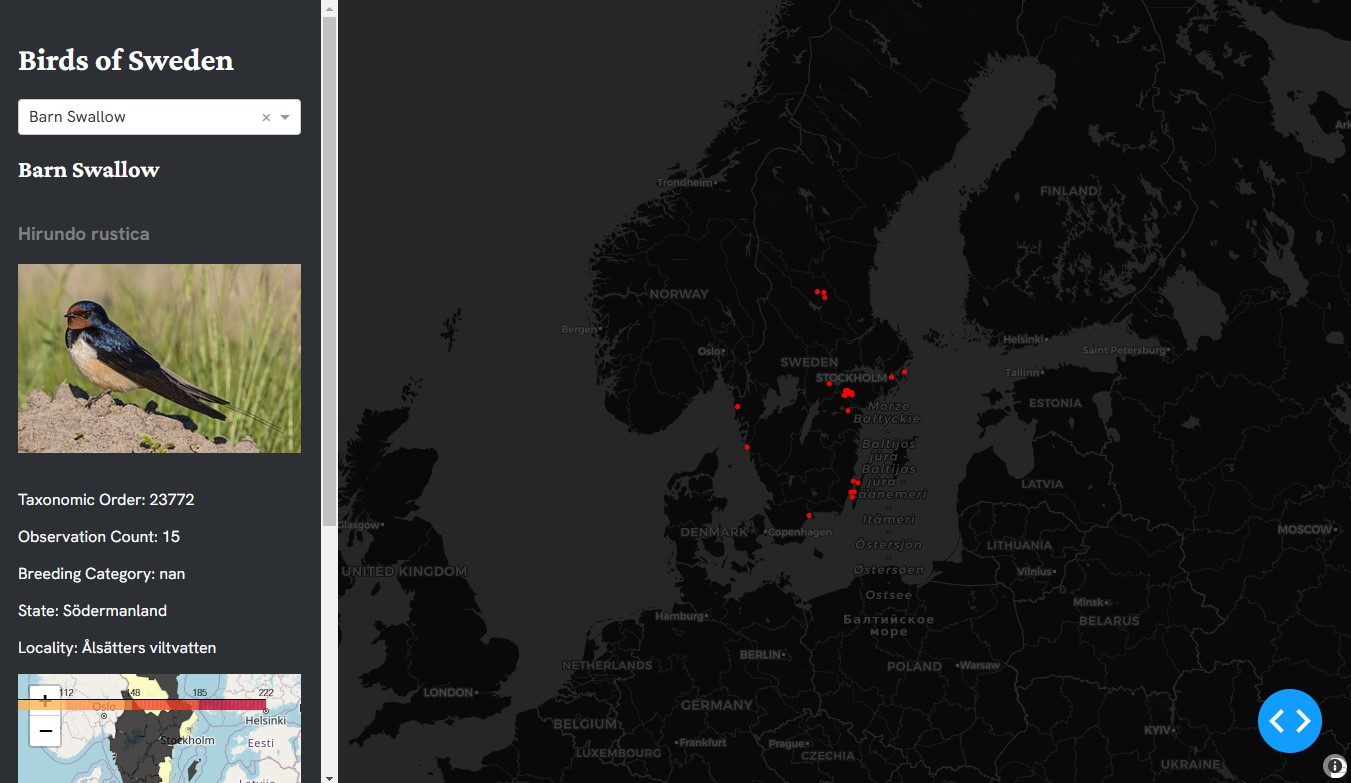
\includegraphics[width=0.8\textwidth]{figures/species_details.jpg} 
    \caption{Map displaying observations of a selected species after filtering.} 
    \label{fig:filtered_map} 
\end{figure}

\subsection{Details on Demand}

To offer in-depth information, the dashboard provides detailed data about specific observations and species. When a species is selected, the sidebar displays:

\begin{itemize} 
    \item \textbf{Species Name and Scientific Name}: Clarifies the common and scientific nomenclature. 
    \item \textbf{Species Image}: Retrieves an image from Wikipedia for visual identification. 
    \item \textbf{Additional Information}: Presents taxonomic order, observation count, breeding category, state, and locality. 
\end{itemize}

This implementation of "Details on Demand" ensures that users can access specific information without overwhelming the initial view. Moreover, clicking on an observation point on the map sets the species in the dropdown, updating the sidebar with relevant details (Figure~\ref{fig:details_on_demand}).

\begin{figure}[h] 
    \centering 
    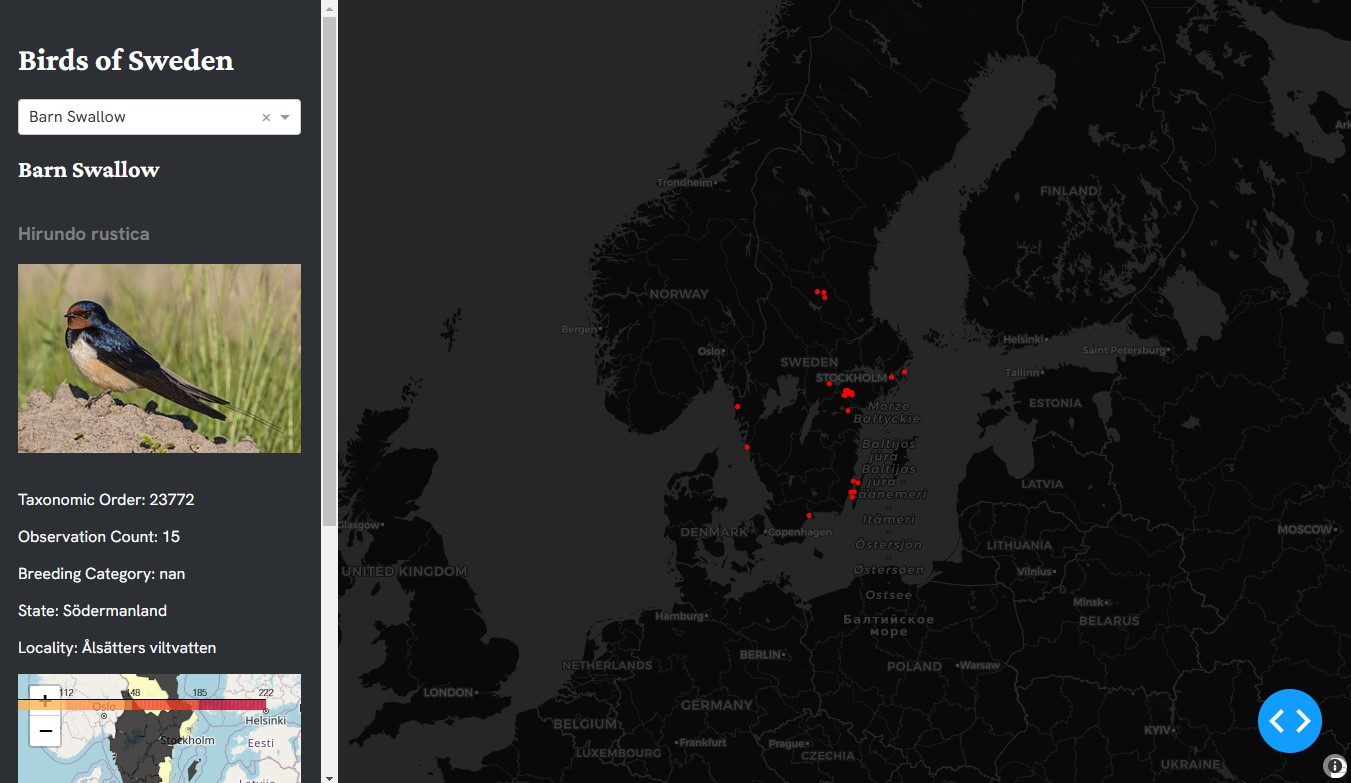
\includegraphics[width=0.4\textwidth]{figures/species_details.jpg} 
    \caption{Detailed information displayed upon species selection.} 
    \label{fig:details_on_demand} 
\end{figure}

\subsection{Technical Implementation}

The dashboard leverages the Dash framework for Python, enabling the creation of interactive web applications. Key implementation aspects include:

\begin{itemize} 
    \item \textbf{Data Loading}: The full dataset is loaded without slicing to ensure all observations and species are available. 
    \item \textbf{Data Cleaning}: Missing values in critical columns such as \texttt{LATITUDE}, \texttt{LONGITUDE}, and \texttt{COMMON NAME} are handled to prevent empty maps or dropdowns. 
    \item \textbf{Callbacks}: Dash callbacks are used to update the map and sidebar components dynamically based on user interactions. 
    \item \textbf{Geographical Consistency}: The state observations map uses the \texttt{fitbounds="geojson"} parameter to always display the entire country's outline, regardless of the data filtered. 
\end{itemize}

By addressing initial issues such as empty maps on startup and mismatches in state naming conventions, the dashboard now aligns with the intended functionality and provides a seamless user experience.

\section{Goals and Hopes for the Dashboard}

The primary objective of implementing Shneiderman's Mantra in the Birds of Sweden Dashboard is to enhance user interaction and facilitate the exploration of bird fauna data. The specific goals include:

\subsection{Improving User Interaction and Experience}

By providing an intuitive interface that adheres to established principles of information visualization, users can navigate the dataset effectively, regardless of their familiarity with the data. The hierarchical approach reduces cognitive load and allows for a more engaging experience.

\subsection{Facilitating Exploration of Sweden's Bird Fauna}

The dashboard serves as an educational tool, enabling users to discover patterns and insights within the bird observation data. For instance, users can identify regions with high biodiversity, track migration patterns, or explore species distribution.

\subsection{Enabling Users to Gain Insights}

Through interactive filtering and detailed information access, users can perform analyses that may lead to new findings or support research efforts. Conservationists, ornithologists, and bird enthusiasts alike can leverage the dashboard to inform their work or interests.

\section{Conclusion}

Implementing Shneiderman's Mantra in the Birds of Sweden Dashboard has resulted in a powerful tool for data exploration. By providing an initial overview, enabling focused filtering, and offering detailed information on demand, the dashboard aligns with best practices in information visualization. The hope is that this approach not only enhances user engagement but also contributes to a deeper understanding of Sweden's rich bird fauna.